\documentclass[a4paper,12pt, oneside]{book}

%\usepackage{fullpage}
\usepackage[italian]{babel}
\usepackage[utf8]{inputenc}
\usepackage{amssymb}
\usepackage{amsthm}
\usepackage{graphics}
\usepackage{amsfonts}
\usepackage{listings}
\usepackage{amsmath}
\usepackage{amstext}
\usepackage{engrec}
\usepackage{rotating}
\usepackage[safe,extra]{tipa}
\usepackage{showkeys}
\usepackage{multirow}
\usepackage{hyperref}
\usepackage{microtype}
\usepackage{enumerate}
\usepackage{braket}
\usepackage{marginnote}
\usepackage{pgfplots}
\usepackage{cancel}
\usepackage{polynom}
\usepackage{booktabs}
\usepackage{enumitem}
\usepackage{framed}
\usepackage{pdfpages}
\usepackage{pgfplots}
\usepackage[cache=false]{minted}

\usepackage{tikz}\usetikzlibrary{er}\tikzset{multi  attribute /.style={attribute ,double  distance =1.5pt}}\tikzset{derived  attribute /.style={attribute ,dashed}}\tikzset{total /.style={double  distance =1.5pt}}\tikzset{every  entity /.style={draw=orange , fill=orange!20}}\tikzset{every  attribute /.style={draw=MediumPurple1, fill=MediumPurple1!20}}\tikzset{every  relationship /.style={draw=Chartreuse2, fill=Chartreuse2!20}}\newcommand{\key}[1]{\underline{#1}}

\usepackage{fancyhdr}
\pagestyle{fancy}
\fancyhead[LE,RO]{\slshape \rightmark}
\fancyhead[LO,RE]{\slshape \leftmark}
\fancyfoot[C]{\thepage}



\title{Basi di Dati}
\author{UniShare\\\\Davide Cozzi\\\href{https://t.me/dlcgold}{@dlcgold}\\\\Gabriele De Rosa\\\href{https://t.me/derogab}{@derogab} \\\\Federica Di Lauro\\\href{https://t.me/f_dila}{@f\textunderscore dila}}
\date{}

\pgfplotsset{compat=1.13}
\begin{document}
\maketitle

\definecolor{shadecolor}{gray}{0.80}
\setlist{leftmargin = 2cm}
\newtheorem{teorema}{Teorema}
\newtheorem{definizione}{Definizione}
\newtheorem{esempio}{Esempio}
\newtheorem{corollario}{Corollario}
\newtheorem{lemma}{Lemma}
\newtheorem{osservazione}{Osservazione}
\newtheorem{nota}{Nota}
\newtheorem{esercizio}{Esercizio}
\tableofcontents
\renewcommand{\chaptermark}[1]{%
\markboth{\chaptername
\ \thechapter.\ #1}{}}
\renewcommand{\sectionmark}[1]{\markright{\thesection.\ #1}}
\chapter{Introduzione}
\textbf{Questi appunti sono presi a ldurante le esercitazioni in laboratorio. Per quanto sia stata fatta una revisione è altamente probabile (praticamente certo) che possano contenere errori, sia di stampa che di vero e proprio contenuto. Per eventuali proposte di correzione effettuare una pull request. Link: } \url{https://github.com/dlcgold/Appunti}.\\
\textbf{Grazie mille e buono studio!}
\chapter{Introduzione al Corso}
Il corso di Basi di Dati affronta gli aspetti e i metodi per lo sviluppo di un database in maniera efficiente,
aspetto fondamentale per un informatico e per lo sviluppo ottimale di software. \newline
Il corso si divide in 7 parti:
\begin{enumerate}
\item introduzione generale
\item metodologie e modelli per il progetto delle basi di dati
\item progettazione concettuale
\item modello razionale
\item progettazione logica
\item linguaggio SQL
\item algebra relazionale
\end{enumerate}
Le \textbf{informazioni} fanno parte delle risorse di un'azienda, soprattuto negli ultimi anni di clima globale,
per cui la gestione efficiente ed ottimale dei dati è fondamentale, come ad esempio Facebook ed Amazon fanno ampio
uso dei nostri dati, sia a scopi pubblicitari sia a scopi di marketing.

Un sistema informativo è una componente di un'organizzazione che gestiste le informazioni d'interesse, non per forza attraverso
un'automatizzazione e/o supporto di un calcolatore, infatti sin dall'antichita le banche 
tenevano traccia dei depositi tramite un archivio cartaceo.

Una porzione automatizzate del sistema informativo si chiama sistema informatico, che si divide in:
\begin{itemize}
    \item acquisizione e memorizzazione
    \item aggiornamento
    \item interrogazione
    \item elaborazione
\end{itemize}
Le informazioni vengono gestite in vari modi, attraverso il linguaggio naturale, graficamente con schemi e/o numeri, 
con il tempo si è arrivati a codifiche standard per quasi tutte le tipologie di informazioni, e sono rappresentate 
nei sistemi informatici dai \emph{dati}, la cui differenza è che i dati sono valori senza alcun valore 
mentre le informazioni stabilisce un'interpretazione attribuendo una semantica ai valori. 

I dati sono una risorsa strategica in quanto sono stabili nel tempo, infatti solitamente i dati sono immutati
durante una migrazione tra un sistema e un altro, per questo lo sviluppo progettazione di un database rimane stabile in teoria,
senza notevoli cambiamenti durante la durata di un sistema informativo.

Un \textbf{Data Base} è una collezione di dati usati per rappresentare le informazioni di interesse di un sistema informativo,
definite solo una volta a cui un insieme di applicazioni ed utenti può accedere ad essi, 
mentre un \textbf{DBMS} è un software per la gestione di un database.

I dati presenti in un database sono molti, indipendenti dal programma in cui vengono utilizzati e cui si cerca di evitare 
la ridondanza, per garantire la consistenza delle informazioni.

Per la creazione di un database, al fine di garantire privatezza, affidabilità, efficienza ed efficacia,
sono presenti le seguenti tre fasi:
\begin{enumerate}
    \item definizione
    \item creazione e popolazione
    \item manipolazione
\end{enumerate}
Un organizzazione è divisa in vari settori e ogni settore ha un suo sottosistema informativo, non necessariamente disgiunto,
e i database solitamente sono condivisi, al fine di ridurre la ridonzanza delle informazioni, per cui sono presenti
meccanismi di autorizzazione e di controllo della concorrenza.\newline
Un database deve essere conservato a lungo termine e si ha una gestione delle \textbf{transazioni}:
insieme di operazioni da considerare indivisibile, atomico, corretto anche in presenza di concorrenza e con effetti definitivi.

La sequenza di operazioni nel database deve essere eseguita nella sua interezza, per cui l'effetto di 
transazioni concorrenti deve essere coerente, infatti la conclusione positiva di una transazioni corrisponde ad un impegno,
\emph{commit}, a mantenere traccia del risultato, anche in presenza di guasti e di esecuzioni concorrente.\newline
Come tutti i software, i DBMS devono essere efficienti, utilizzando al meglio memoria e tempo, efficaci e produttivi.

Si hanno delle caratteristiche nell'approccio alla base dati:
\begin{itemize}
    \item natura autodescrittiva di un sistema di basi di dati: il sistema di basi di dati memorizza i dati con
          anche una descrizionie completa della sua struttura(metadati), per consentire ai DBMS di lavorare con qualsiasi applicazione.
    \item separazione tra programmi e dati, infatti è possibile cambiare la struttura dati senza cambiare i programmi.
    \item astrazione dei dati: si usa un modello dati per nascondere dettagli e presentare
            all'utente una visione concettuale del database.
    \item supporto di viste multiple dei dati, per cui ogni utente può usare una vista (view) differente del
          database, contenente solo i dati di interesse per quell'utente.
    \item condivisione dei dati e gestione delle transazioni con utenti multipli.
\end{itemize}
I DBMS estendono le funzionalità dei file system, fornendo più servizi ed in maniera integrata.

In ogni base di dati si ha:
\begin{itemize}
    \item lo \textbf{schema}, sostanzialmente invariante nel tempo, che ne descrive la struttura, l'aspetto intensionale.
    \item l'\textbf{istanza}, i valori attuali, che possono cambiare anche molto rapidamente, l'aspetto estensionale "concreto".
\end{itemize}
Per lo sviluppo delle basi di dati si hanno due tipi di modelli, ambedue importanti:
\begin{itemize}
    \item \textbf{modelli logici}, adottati nei DBMS esistenti per l'organizzazione dei dati, 
            utilizzati dai programmi e sono indipendenti dalle strutture fisiche
    \item \textbf{modelli concettuali} che permettono di rappresentare i dati in modo indipendente da ogni sistema,
            con il fine di descrivere i concetti del mondo reali;sono usati nelle fasi preliminari di progettazione 
            e il più diffuso è il modello \textbf{Entity-Relationship}.
\end{itemize}
%immagine architettura standard
Un database è organizzato solitamente attraverso i tre schemi dell'architettura ANSI/SPARC:
\begin{enumerate}
        \item [schema logico:] descrizione dell'intera base di dati nel modello logico “principale” del DBMS,
                ossia si definisce la struttura concettuale del database, 
                senza considerare l'implementazione fisica nel DBMS.
        \item [schema fisico:] rappresentazione dello schema logico per mezzo di strutture fisiche di memorizzazione
        \item [schema esterno:] descrizione di parte della base di dati in un modello logico
                (“viste” parziali, derivate, anche in modelli diversi)
\end{enumerate}
L'accesso ai dati avviene solo mediante il livello esterno, il quale a volte coincide con quello logico, 
e si hanno 2 forme di indipendenza: quella fisica, in cui è possibile interagire con il DBMS senza conoscere la struttura fisica
e quella logica, in cui si può accedere al livello esterno senza interagire con lo schema logico.

Per la definizione dei database ci sono quattro tipologie di linguaggi:
\begin{itemize}
        \item \textbf{DLL}(Data Manipulation Languages) linguaggio per definire i dati
        \item \textbf{DML}(Data Manipulation Languages) linguaggio per la manipolazione dei dati
        \item \textbf{DCL}(Data Control Languages) linguaggio per il controllo degli accessi al database
        \item \textbf{DQL}(Data Query Languages) linguaggio per effettuare delle interrogazioni al database
\end{itemize}
Noi vedremo SQL per definire i database, linguaggio basato sull'algebra relazionale che implementa tutti e 4 le tipologie 
di linguaggi per la gestione di un database.

Si hanno due tipi di utenti:
\begin{enumerate}
    \item \textbf{utenti finali (terminalisti):} eseguono applicazioni predefinite (transazioni)
    \item \textbf{utenti casuali:} eseguono operazioni non previste a priori, usando linguaggi interattivi
\end{enumerate}
inoltre si hanno:
\begin{itemize}
    \item progettisti e realizzatori di DBMS
    \item progettisti della base di dati e amministratori della base di dati (DBA), 
          persona o gruppo di persone responsabile del controllo centralizzato del database,
          in tutti i suoi aspetti.
    \item progettisti e programmatori di applicazioni
\end{itemize}
\begin{center}
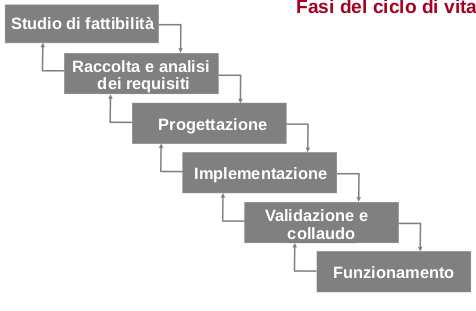
\includegraphics[scale=0.8]{img/bas.png}
\end{center}
Come visto anche nel corso di analisi e progettazione del software e nella figura X,
durante lo sviluppo di un sistema informatico si hanno le seguente fasi:
\begin{itemize}
    \item \textbf{studio di fattibilità}, definizione di costi, priorità e competenze per un progetto
    \item\textbf{raccolta e analisi dei requisiti}, ovvero lo studio delle proprietà del sistema
    \item \textbf{progettazione} di dati e funzioni
    \item \textbf{implementazione}
    \item \textbf{validazione e collaudo},che comprendono anche test da parte del cliente
    \item \textbf{funzionamento}, ovvero lo stadio finale dove il sistema diventa effettivamente operativo
\end{itemize}
In questo corso ci occuperemo soltanto delle fasi di progettazione ed implementazione di base di dati, 
lasciando l'analisi delle altre fasi al corso ed ai libri di Ingegneria del Software.\newline
In questo processo a rimanere stabili sono prettamente i \textbf{dati} infatti prima si progetta la base dati,
con una \textbf{metodologia di progetto}, e poi il software.
\begin{center}
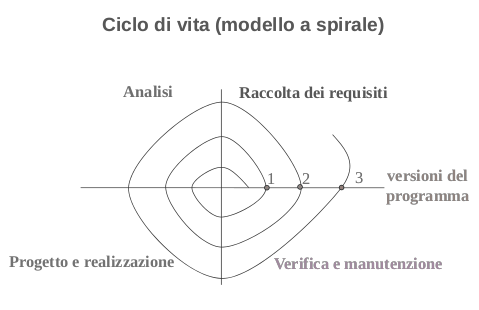
\includegraphics[scale=2.8]{img/bas2.png}
\end{center}
Una \textbf{metodologia} è un'articolazione in fasi di guida ad un'attività di progettazione, in caso
di una base dati la metodologia, con il fine di separare il cosa rappresentare dal come, è la seguente:
\begin{itemize}
    \item suddivida la progettazione in fasi indipendenti
    \item fornisca strategie e criteri di scelta in caso di alternative
    \item fornisca modelli di riferimento (i linguaggi)
    \item garantisca generalità rispetto al problema
    \item garantisca qualità e facilità d'uso
\end{itemize}
\begin{center}
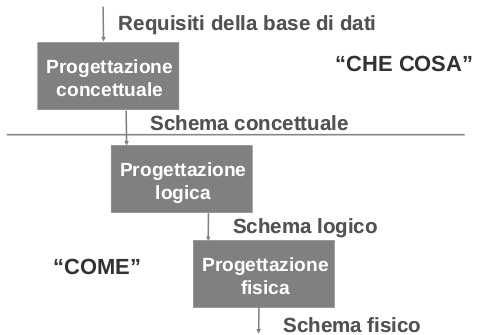
\includegraphics[scale=2.5]{img/bas3.png}
\end{center}
\begin{center}
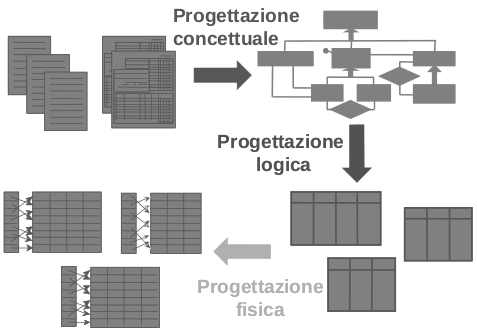
\includegraphics[scale=2.5]{img/bas4.png}
\end{center}
Come si può notare nella figura X1, la metodologia corrente di modellazione di un database
prevede la definizione e l'esecuzione delle seguenti fasi:
\begin{itemize}
    \item la \textbf{progettazione concettuale} consiste nel tradurre i requisiti del sistema informatico
            in una descrizione formale, integrata e indipendente dalle scelte implementative (DBMS, SW e HW)
    \item la \textbf{progettazione concettuale} consiste nella traduzione dello schema concettuale nel modello dei dati
            scelto per la modellazione, ottenendo uno schema logico, espresso nel DDL del DBMS.\newline
          In questa fase si considerano anche aspetti legati ai vincoli ed all'efficienza. Si hanno due sotto-fasi:
          \begin{itemize}
                \item ristrutturazione dello schema concettuale
                \item traduzione verso il modello logico
          \end{itemize}
    \item la \textbf{progettazione fisica} completa lo schema logico ottenuto con le specifiche proprie del DBMS scelto.
          Il risultato è lo schema fisico che descrive le strutture di memorizzazione ed accesso ai dati
\end{itemize}
Incominciamo nel prossimo capitolo a considerare la progettazione concettuale, per poi analizzare nei successivi capitolo
in dettaglio anche la fase di progettazione concettuale e il linguaggio SQL.

\chapter{Progettazione Concettuale:ER}
Come abbiamo già introdotto nel precedente capitolo, affrontiamo ora la progettazione concettuale di una base dati attraverso
il modello \textbf{ER}(Entity Relationships), modello concettuale che fornisce una serie di strutture
atte a descrivere in maniera semplice e facile la realtà di interesse da modellare.

Si hanno dei vantaggi con la progettazione concettuale, prevale infatti l'aspetto intensionale indipendente
dalla tecnologia ed è una rappresentazione grafica ed è utile per la documentazione, in quanto facilmente comprensibile anche
da persone poco avezze alla tecnologia e ai database.

In uno schema ER si hanno i seguenti costrutti, come si nota nella figura Y,
la cui rappresentazione effettiva varia in quanto vi sono più versioni di ER:
\begin{itemize}
        \item \textbf{entità}: classe di oggetti con proprietà comune ed esistenza "autonoma", della quale si vogliono specificare 
              fatti specifici;ogni entità ha un nome univoco, espressivo e al singolare.
      \item \textbf{relazione}: rappresentano legami logici, significativi per la realtà da modellare, tra due o più entità.\newline
            Un'occorrenza di relazione è un n-upla costituita da occorrenze di entità, una per ciascuna delle entità coinvolte,
          e ogni relazione ha un nome univoco, in cui è preferibile assegnare un sostantivo per evitare di stabilire un verso alla relazione.\\
          Essendo una relazione matematica tra le entità coinvolte non è possibile avere delle n-uple identiche, con conseguenze
          per la realtà da rappresentare, per esempio non è possibile attraverso una relazione il fatto che è possibile 
          ripetere un esame, obbligando a rappresentare l'esame come entità e non più come relazione.
  \item \textbf{attributo semplice}: associa ad ogni istanza di entità o associazione un valore, definito su un dominio di valori,
          specificato nella documentazione associata, con il fine di descrivere le proprietà elementari 
          di entità e/o relazioni disegnate per rappresentare la realtà d'interesse.\newline
  \item \textbf{attributo composto}: raggruppamento di attributi di una medesima entità/relazione con affinità di significato e/o uso
          come ad esempio possiamo raggruppare gli attributi Via, Numero Civico e Cap dall'entità persona per formare 
          l'attributo composto Indirizzo.
  \item \textbf{cardinalità delle relazioni}: vengono specificate per ogni relazione e descrivono il numero minimo e massimo di occorrenze
            di relazione, a cui una occorrenza dell'entità può partecipare alla relazione, ossia quante volte un'occorrenza 
            di un'entità può essere legata ad occorrenze delle altre entità coinvolte.\newline
          È possibile assegnare un qualunque intero non negativo, con l'unico vincolo che la cardinalità minima 
          sia minore o uguale alla cardinalità massima e di solito si usano i valori $0, 1 \text{e} N$, indicanti
          zero, una o molte occorrenze, senza preoccuparsi in caso di $N$ del numero effettivo di occorrenze.
  \item \textbf{cardinalità di un attributo}: descrivono il numero minimo e massimo di valori dell'attributo 
            associati all'entità e/o relazione, con la cardinalità $(1, 1)$ stabilita come default,
          che può essere vista come funzione che associa ad ogni occorenza di entitò un solo valore dell'attributo;
          si hanno le stesse consetutidini delle cardinalità delle relazioni.
  \item \textbf{identificatore interno}: permette di identificare in maniera univoca un'entità ed un identificatore è interno
          in caso sia uno o più attributi di un'entità, tutti con cardinalità $(1, 1)$.
  \item \textbf{identificatore esterno}: un identificatore è esterno, in caso un'entità $E$  viene identificata da un'attributo
          di un'entità $F$, cui esiste una relazione uno a uno tra l'entità $E$ e $F$.\newline
          È possibile, anche se molto raro, avere la definizione dell'identificatore usando entità di entità, ossia 
          l'identificatore dell'entità $E$ viene definito nell'entità $G$, cui esiste una relazione con l'entità $F$
          che a sua volta ha una relazione con l'entità $E$, ma si può capire da quanto è contorto il ragionamento 
          qual'è la sua percentale d'utilizzo nella modellazione dello schema ER.
  \item \textbf{generalizzazione}: rappresentano legami logici tra un entità $E$, detta padre, e una serie di entità $E_1, E_2, \dots, E_n$,
          dette figlie, di cui l'entità $E$ rappresenta un caso generale della serie di entità figlie.\newline
          Tra le entità coinvolte in una generalizzazione valgono le seguenti proprietà:
          \begin{itemize}
            \item ogni occorrenza di un'entità figlia è anche un'occorrenza dell'entità genitore.
            \item ogni proprietà dell'entità genitore è anche una proprietà delle entità figlie, quindi
                  nello schema ER non devono essere rappresentate, e ciò prende il nome di ereditarietà.
          \end{itemize}
          Le generalizzazioni possono essere classificate sulla base di due proprietà ortogonali:
          \begin{itemize}
            \item una generalizzazione è totale se ogni occorrenza del genitore è un occorrenza di almeno
                  uno dei figli, altrimenti è parziale.
            \item una generalizzazione è esclusiva se ogni occorrenza del genitore è al più un'occorrenza 
                  di una delle entità figlie, altrimenti è sovrrapposta.
          \end{itemize}
  \item \textbf{sottoinsieme}: generalizzazione con soltanto un entità figlia, di cui solitamente rappresenta una parte 
            dell'entità genitore come ad esempio gli studenti sono un sottoinsieme delle persone.
\end{itemize}

\begin{figure}
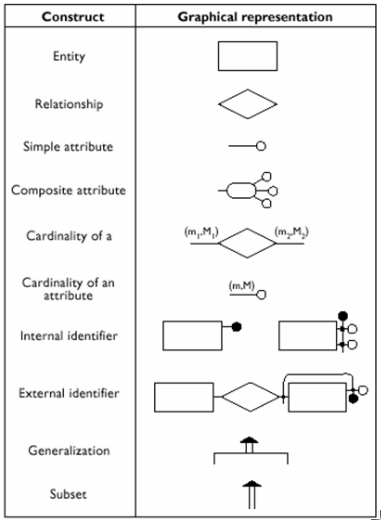
\includegraphics[scale=0.8]{img/bas6.png}
\end{figure}
Un'occorrenza, o istanza, di un'entità, è un oggetto della classe che l'entità rappresenta,
ma noi rappresentiamo le entità dello schema concettuale non le singole istanze, in quanto esse
sono variabili nel tempo a differenza della struttura, concetto fondamentale per definire un modello funzionale.

Nessuno impone un tipo per un certo attributo, possono essere anche complessi di cui però non ci interessano le informazioni
che lo rappresentano, come ad esempio una foto può essere un attributo, ma se ho bisogno dell'autore della foto,
non sarà più un attributo ma un'altra entità. 

Un'\textbf{istanza di associazione} è una combinazione o aggregazione di istanze di entità che prendono
parte all'associazione (per esempio "prof. Schettini" è istanza di associazione per l'entità docente).\newline
Le relazioni possono avere attributi, con valori specificati in un certo dominio, che  modella una proprietà del legame
tra tutte le entità rappresentato dalla relazione.

Una associazione può coinvolgere “due o più volte” la stessa entità e ciò si chiama \emph{associazione ricorsiva o ad anello},
come si nota nella figura XXXX, ed è molto utile per definire le relazioni subordinazione e/o comunicazioni tra istanze
di una stessa entità, come nel caso della relazione sovrano, indicante la lista dei sovrani con i predecessori e successori;
in queste associazioni è necessario aggiungere la specifica dei \textbf{ruoli}, come nell'esempio SDERR, per specificare
in maniera chiara e non ambigua quale è il verso della relazione.

Un'associazione ad anello, ovviamente essendo una relazione, può avere delle proprietà come ad esempio la relazione della figura
SJDFHJF è irriflessiva, intransitiva e asimetrica.

\begin{figure}
\centering
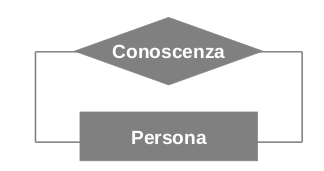
\includegraphics[scale=2.5]{img/bas7.png}
\end{figure}

\begin{center}
    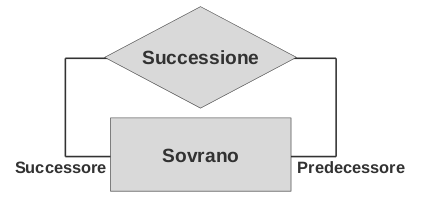
\includegraphics[scale=2.5]{img/bas8.png}
\end{center}

\newpage
\textit{Descrivere lo schema concettuale della seguente
realtà:
I docenti hanno un codice fiscale ed una età. I
docenti operano nei corsi di laurea (si dice che
afferiscono ai corsi di laurea). Interessa la data di
afferenza dei docenti ai corsi di laurea. I corsi di
laurea hanno un codice ed un nome, ed
appartengono alle facoltà. Ogni facoltà ha un nome}
\begin{center}
\begin{tikzpicture}[node  distance =7em]
\node[entity] (docente) {docente};
\node[attribute] (età) [above left of =  docente] {età} edge (docente);
\node[attribute] (codice) [above of = docente] {codice fiscale} edge (docente);
\node[relationship] (operatore) [right of = docente] {operatore} edge (docente);
\node[attribute] (data) [below of = operatore ] {data} edge (operatore);
\node [entity] (laurea) [right of = operatore] {laurea} edge (operatore);
\node[attribute] (cod) [above of =  laurea] {nome} edge (laurea);
\node[attribute] (nome) [above right of = laurea] {codice} edge (laurea);
\node[relationship] (appartenenza) [below of = laurea] {appartenenza} edge (laurea);
\node [entity] (facoltà) [below of = appartenenza] {facoltà} edge (appartenenza);
\node[attribute] (nomee) [below of = facoltà] {nome} edge (facoltà);
\end{tikzpicture}
\end{center}
\newpage
\begin{esempio}
Descrivere lo schema concettuale della seguente
realtà:
Degli impiegati interessa il codice fiscale, il nome, il
cognome, i dipartimenti ai quali afferiscono (con la
data di afferenza), ed i progetti ai quali partecipano.
Dei progetti interessa il nome, il budget, e la città in
cui hanno luogo le corrispondenti attività. Alcuni
progetti sono parti di altri progetti, e sono detti loro
sottoprogetti. Dei dipartimenti interessa il nome, il
numero di telefono, gli impiegati che li dirigono, e la
città dove è localizzata la sede. Delle città interessa
il nome e la regione:
\begin{center}
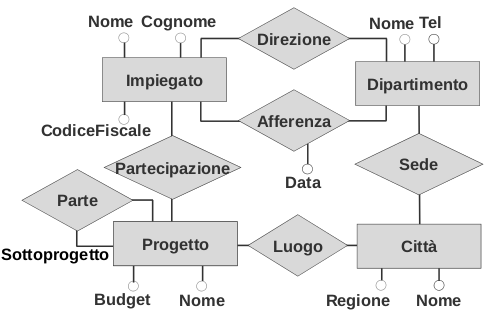
\includegraphics[scale=3]{img/er.png}
\end{center}
\end{esempio}
Nella scelta del costrutto ideale, per rappresentare in maniera fedele e corretta la realtà, si usano le seguenti "regole":
\begin{itemize}
    \item \textbf{entità}: si usa un entità in caso vengano rispettate le seguenti proprietà: 
          le sue istanze sono significative indipendentemente dalle altre istanze, se si ha o si può avere delle proprietà
                indipendenti dagli altri concetti oppure se il concetto da rappresentare è importante per la realtà da modellare.
                
    \item \textbf{attributo}: si usa un'attributo in caso succedono i seguenti avvenimenti: non ha senso
            considerare una sua instanza a se stante ad altre instanze, le istanze non sono concettualmente significative
            oppure serve soltanto rappresentare una proprietà locale di un altro concetto.

    \item \textbf{relazione}: si dovrebbe usare una relazione in caso non ha senso pensare alla partecipazione
            delle sue instanze ad altre relazioni e le sue istanze non sono significative indipendentemente da altre istanze,
                ossia una sua istanza ha senso se messa in relazione con altre istanze, provenienti da altri costrutti.

\end{itemize}

\begin{center}
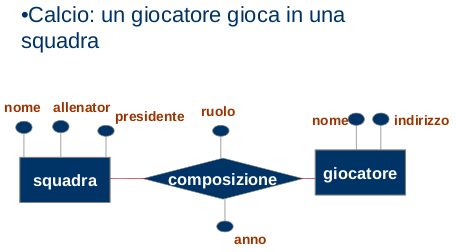
\includegraphics[scale=1]{img/er2.png}
\end{center}
\begin{esempio}
\begin{itemize}
\item ogni zoo è diviso in aree diverse a seconda che si tratti di rettili, pesci, uccelli, scimmie, grandi mammiferi, ... Ogni area è dotata di: nome,
indirizzo, dimensione, numero di sezioni.
\item per ogni tipo di animale ci sono informazioni che riguardano: classificazione zoologica, nome comune (giraffa, elefante, serpente,
tartaruga, ...), habitat, alimentazione, ... Per ogni tipo di animale c'è un diverso veterinario specialista, dipendente dello zoo.
\item ogni tipo di animale è rappresentato da esemplari e relativi dati anagrafici: nome proprio (giraffa Enrico, giraffa Giulia, ...), data di nascita,
Paese di provenienza, data di arrivo allo zoo, ...
\item ogni esemplare è dotato di più schede sanitarie contenenti ognuna: la data della visita, referto, dieta, nome del veterinario, ...

\end{itemize}
\begin{center}
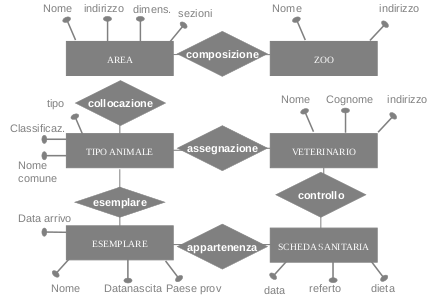
\includegraphics[scale=0.8]{img/er3.png}
\end{center}
lo zoo ha degli attributi che vanno indicati anche se non richiesti dalla traccia per evitare ambiguità. Dato che ogni scheda è collegata ad un veterinario, di cui ho un'entità la collego a veterinario con una relazione e non ne faccio  un attributo
\end{esempio}
\begin{center}
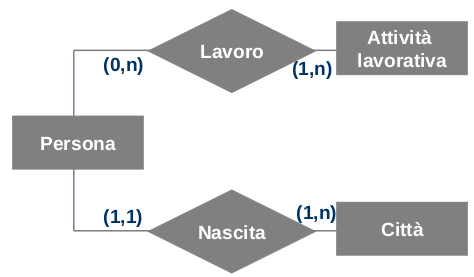
\includegraphics[scale=0.8]{img/er4.png}
\end{center}
\begin{center}
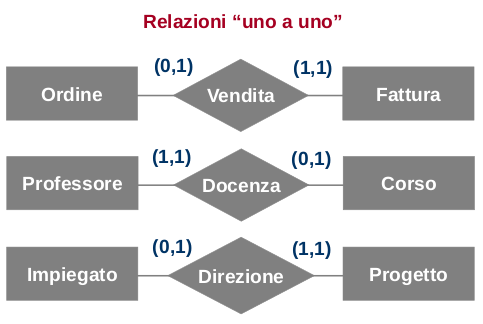
\includegraphics[scale=0.6]{img/er7.png}
\end{center}
\begin{center}
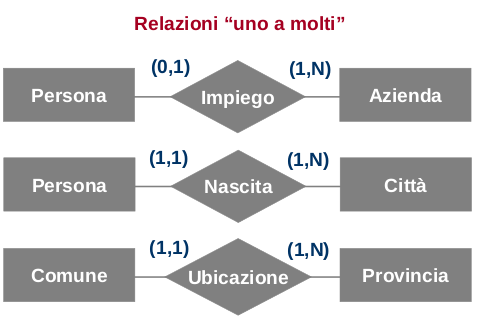
\includegraphics[scale=0.6]{img/er6.png}
\end{center}
\begin{center}
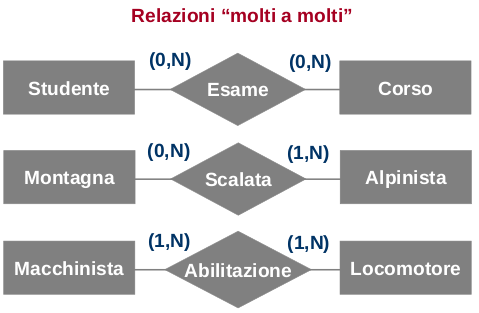
\includegraphics[scale=0.6]{img/er5.png}
\end{center}
vediamo un esempio:
\begin{esempio}
si ha:
\begin{center}
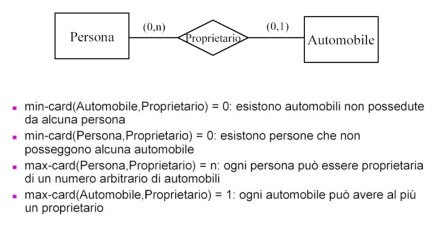
\includegraphics[scale=0.8]{img/er8.png}
\end{center}

\end{esempio}
\begin{center}
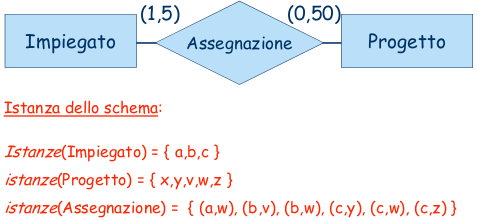
\includegraphics[scale=0.8]{img/er9.png}
\end{center}
\textit{Ad ogni impiegato sono assegnati da 1 a 5 progetti e ogni progetto è assegnato ad al più 50 impiegati. a,b,c compaiono in almeno una istanza di Assegnazione. x non compare nelle istanze di Assegnazione. Infine ci sono progetti (ad esempio lanciati da poco
tempo) che possono non essere assegnati a nessun
impiegato}\\
\begin{center}
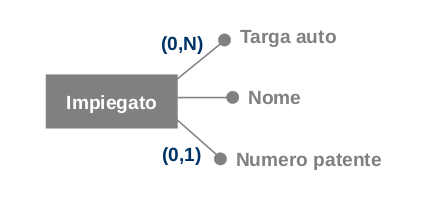
\includegraphics[scale=0.8]{img/er10.png}
\end{center}
\begin{center}
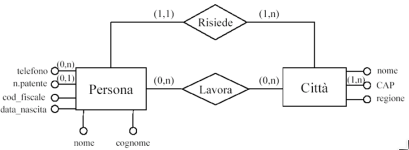
\includegraphics[scale=0.8]{img/er11.png}
\end{center}
\begin{center}
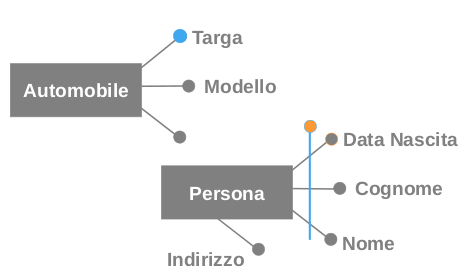
\includegraphics[scale=0.8]{img/er12.png}
\end{center}
\begin{center}
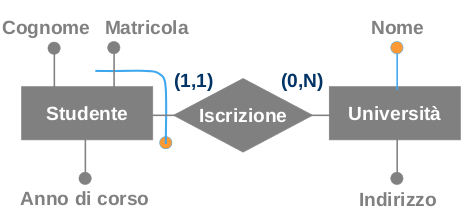
\includegraphics[scale=0.8]{img/er13.png}
\end{center}
vediamo un esempio complesso, che è preso da un vecchio esempio:
\begin{center}
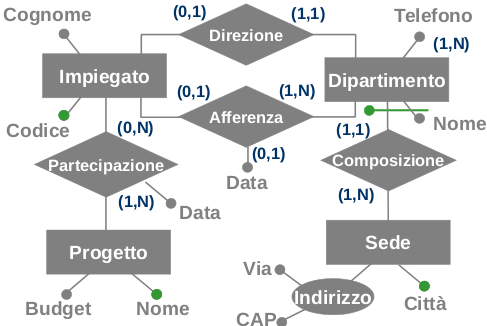
\includegraphics[scale=0.8]{img/er14.png}
\end{center}
\subsection{Relazione IS-A}
È facile verificare che, in molti contesti, può
accadere che tra due classi rappresentate da due
entità nello schema concettuale sussista la relazione
IS-A (o relazione di sottoinsieme), e cioè che ogni
istanza di una sia anche istanza dell'altra. La relazione IS-A nel modello ER si può definire tra
due entità, che si dicono \textit{entità padre} ed \textit{entità figlia} (o sottoentità, cioè quella che rappresenta un sottoinsieme della entità padre). La relazione IS-A si rappresenta con una freccia dalla sottoentità alla entità padre:
\begin{center}
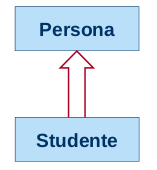
\includegraphics[scale=0.8]{img/isa.png}
\end{center}
Si ha il \textbf{principio di ereditarietà:} \textit{ogni proprietà dell'entità padre è
anche una proprietà della sottoentità, e non si riporta
esplicitamente nel diagramma. L'entità figlia può avere
ovviamente ulteriori proprietà}.\\
Finora, abbiamo considerato la relazione ISA che stabilisce
che l'entità padre è più generale della sottoentità. Talvolta, però, l'entità padre può generalizzare diverse sottoentità rispetto ad un unico criterio. In questo caso si parla di \textbf{generalizzazione}. Nella generalizzazione, le sottoentità hanno insiemi di istanze
disgiunti a coppie (anche se in alcune varianti del modello ER, si può specificare se due sottoentità della stessa entità padre sono disgiunte o no). Una generalizzazione può essere di due tipi:
\begin{enumerate}
\item \textbf{completa:} l'unione delle istanze delle sottoentità è uguale all'insieme delle istanze dell'entità padre
\item \textbf{non completa}
\end{enumerate}
Si dice che:
\begin{itemize}
\item $E$ è \textbf{generalizzazione} di $E_1,\cdots, E_n$
\item $E_1,\cdots,E_n$ sono \textbf{specializzazioni (o sottotipi)} di $E$
\end{itemize}
\newpage
La generalizzazione si indica collegando mediante un arco le
sottoentità, e collegando con una freccia tale arco alla entità padre. La freccia è annerita se la generalizzazione è
completa:
\begin{center}
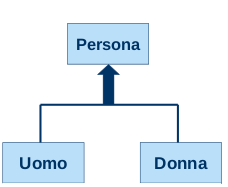
\includegraphics[scale=2.5]{img/isa2.png}
\end{center}
La freccia è non è annerita se la generalizzazione non è
completa:
\begin{center}
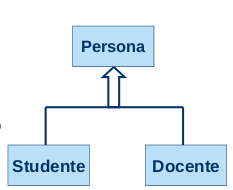
\includegraphics[scale=2.5]{img/isa3.png}
\end{center}
Il principio di ereditarietà vale anche per le generalizzazioni:\textit{ogni proprietà dell'entità padre è anche una proprietà della sottoentità, e non si riporta esplicitamente nel diagramma. L'entità figlia può avere ovviamente ulteriori proprietà:}
\begin{center}
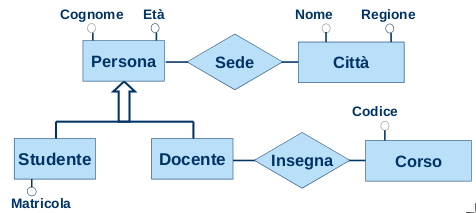
\includegraphics[scale=0.5]{img/isa4.png}
\end{center}
Si hanno delle proprietà per le generalizzazioni. Se $E$, il genitore, è generalizzazione delle figlie $E_1,\cdots, E_n$ si ha:
\begin{itemize}
\item ogni proprietà di $E$ è significativa per $E_1,\cdots, E_n$
\item ogni occorrenza di $E_1,\cdots, E_n$ è occorrenza anche di $E$ 
\end{itemize}
per esempio:
\begin{center}
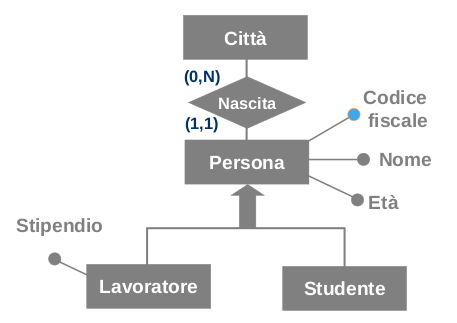
\includegraphics[scale=0.8]{img/isa5.png}
\end{center}
La stessa entità può essere padre in diverse
generalizzazioni. Concettualmente, non c'è alcuna correlazione tra due generalizzazioni diverse, perché rispondono a due criteri diversi di classificare le istanze della entità padre:
\begin{center}
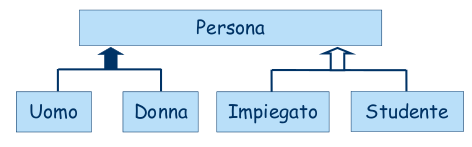
\includegraphics[scale=0.8]{img/isa6.png}
\end{center}
Si possono avere comunque sottoentità indipendenti, nel senso che il loro significato non deriva dallo stesso
criterio di classificazione delle istanze della entità padre:
\begin{center}
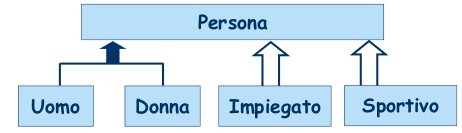
\includegraphics[scale=0.8]{img/isa7.png}
\end{center}
Tutte le proprietà (attributi, relationship,
altre generalizzazioni) dell'entità genitore
vengono ereditate dalle entità figlie e non
rappresentate esplicitamente.\\
Si hanno anche altre proprietà:
\begin{itemize}
\item possono esistere gerarchie a più livelli e
multiple generalizzazioni allo stesso livello
\item un'entità può essere inclusa in più gerarchie,
come genitore e/o come figlia
\item se una generalizzazione ha solo un'entità figlia
si parla di sottoinsieme
\end{itemize}
Alcune interrelazioni non possono essere
colte direttamente da uno schema ER. Tali interrelazioni vanno in ogni caso tenute presenti
attraverso delle asserzioni aggiuntive dette vincoli
esterni al diagramma, o semplicemente vincoli
esterni. Questi vincoli possono essere rappresentati con:
\begin{itemize}
\item formalismi opportuni (es, in
logica matematica)
\item asserzioni in linguaggio
naturale (che devono essere il più possibile
precise e non ambigue)
\end{itemize}
vediamo un esempio. Si ha il seguente schema concettuale:
\begin{center}
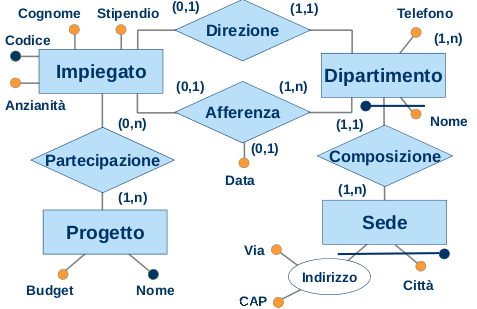
\includegraphics[scale=2.5]{img/vin.png}
\end{center}
con dei vincoli esterni:
\begin{center}
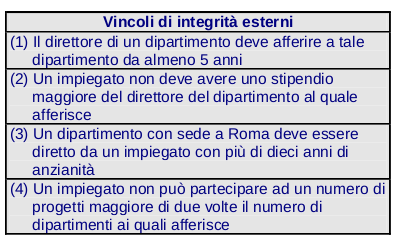
\includegraphics[scale=0.7]{img/vin2.png}
\end{center}
si ottiene:
\begin{center}
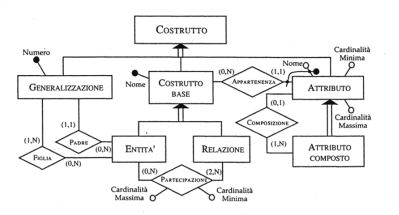
\includegraphics[scale=0.8]{img/vin3.png}
\end{center}

\end{document}
